\documentclass{report}

\usepackage[utf8]{inputenc}
\usepackage{graphicx}
\usepackage[T1]{fontenc}
\usepackage[francais]{babel}%langue française



\begin{document}

\setcounter{page}{0} % enlever numéro de page 
 
\begin{minipage}{0.6\linewidth} % permet de faire les deux colonnes pour mettre l'image à droite du texte
\textbf{Université de Caen Basse-Normandie}\\ 
U.F.R. Sciences \\
Département Informatique\\
Année 2017-2018
\end{minipage}
\begin{minipage}{0.5\linewidth}
\begin{flushright}
	
\includegraphics[scale=0.1]{images/logo.png}
\end{flushright}
\end{minipage}
 
 
\vspace{8cm}
 
 
\begin{center}
\huge \textbf{RAPPORT DU DEVOIR DE TAQUIN }\\

\end{center}
 
 
\vspace{5cm}
 
 
\noindent % permet d'enlever l'indentation du paragraphe
\textbf{Réalisé par :} Abdoulaye BALDE  \\ Mamadou Aliou BAH  \\ Bojan STEFANOVSKI \\ Borjan STOJCHEV


%Création d'une nouvelle page
	\newpage

	%Création de la table des matières
	\tableofcontents

	\newpage

\section{Introduction}
	L'objectif du projet est d'utiliser les connaissances acquises au cours de Complément de POO pour réaliser un projet en Java.
	
	\begin{center}
	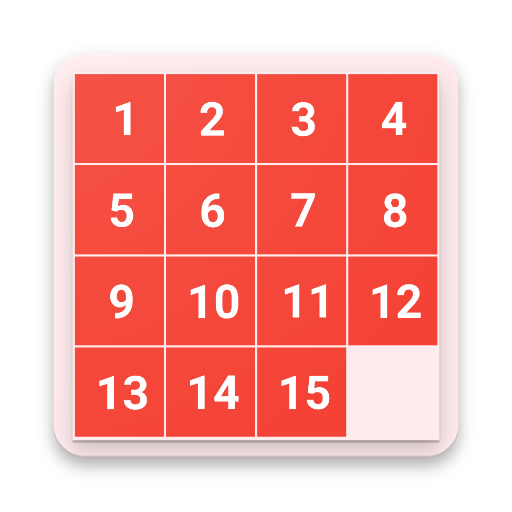
\includegraphics[scale=0.2]{images/taquin.png}
	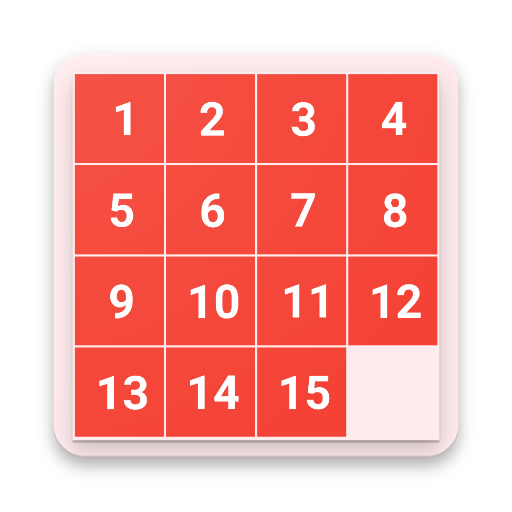
\includegraphics[scale=0.2]{images/taquin.png}
	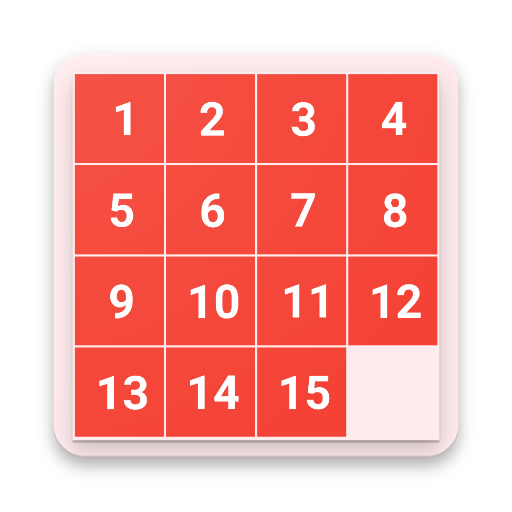
\includegraphics[scale=0.2]{images/taquin.png}
\end{center}
	
	 Le projet consiste a réaliser un jeu de Taquin en utilisant le design pattern MVC, un jeu dotee d'une interface graphique (mais pouvant etre utilise sans l'interface graphique) qui consiste en un puzzle a glissiere. 
	 
	\section{Regles de jeu}
	Le jeu de taquin, parfois aussi appelé le pousse-pousse, est un jeu de réflexion dont le but est de ranger les nombres de 1 à 15 (ou parfois de reconstituer une image) simplement en les faisant glisser.

	\section{Conception}
		Nous avons réalisé l'application integralement MVC, avec modèle totalement independant de l'interface graphique. Le jeu est jouable en ligne de commande et contrôle au clavier (avec les touches h,b,d et g par exemple). Après nous avons implémenté une interface graphique contrôlable par le clavier et la souris.
\newpage		
		\subsection{Diagrammme de classe}
\begin{figure}[ht]
  \includegraphics[scale=0.3]{images/diagramme}
  \caption{Détail des \emph{classes} de Objets}
  \label{fig:packages}
\end{figure}

	\subsection{Partie MVC}
		\begin{itemize} 
		

			\item La classe \textbf{ModelPuzzle} représente notre Observable;
			\item les classes \textbf{Console} et \textbf{Graphique} représente nos Observer, ces classes ne font qu'observer le modèle;
			\item la classe \textbf{Clavier} représente le contrôleur. 
					
		\end{itemize}
		
	
	\section{Problèmes rencontrés}
		Au cours de la réalisation du projet on a rencontré quelques problèmes comme:
		\begin{itemize}
			\item le choix de la représentation des pièces;
			\item le mélange des pièces dans le plateau du jeu. 
		\end{itemize}
		 
				 
	\section{Conclusion}
			Grâce à ce projet nous avons apprit plein de nouvelles connaissances. Il nous a permis à mettre en œuvre le MVC dans un projet. Ce projet nous a également permis de mettre en pratique nos idées pour la conception du jeu de Taquin. 
			
			\subsection{Amélioration}
				Nous projetons d’implémenter une IA pour la résolution automatique du taquin. 
		
	

\end{document}
